%!TEX root = stoh_modeling.tex
\section{Модель}

В данной работе будут рассмотрены 5 основных видов реакций в процессе экспрессии генов:
\begin{itemize}
  \item Присоединение и отсоединение транскрипционных факторов (Рис. \ref{fig:geene_exp1})
  \item Начало транскрипции (Рис. \ref{fig:geene_exp2})
  \item Трансляция (Рис. \ref{fig:geene_exp2})
  \item Деградация белка и тф (Рис. \ref{fig:geene_exp3})
  \item Диффузия между ядрами (Рис. \ref{fig:geene_exp3})
\end{itemize}

\subsection{Транскрипционные факторы}

Наиболее важную роль в экспрессии генов играет присоединение транскрипционных факторов. Связывание происходит к специфичным участкам ДНК - сайтам. Основным
вкладом транскрипционных факторов в экспрессию генов является запуск процесса транскрипции. В данной работе будет предполагаться, что транскрипционные факторы
самостоятельно взаимодествуют, а не в комлексе. Стоит отметить, что для каждого белка свои сайты присоединения на ДНК, которые измевстны из
экспериментальных расчётов.

Транскрипционные факторы делятся на два типа:
\begin{itemize}
  \item \textbf{Активаторы} - белки, которые активируют процесс транскрипции. В нашей работе это будут - \textbf{cad} и \textbf{bcd}.
  \item \textbf{Репрессоры} - белки, которые останавливают процесс транскрипции. В нашей работе это будут - \textbf{tll}, \textbf{hkb}, \textbf{hb},
   \textbf{Kr}, \textbf{gt}
\end{itemize}

Таким образом в экспрессии генов будут задействованы 7 транскрипционных факторов - \textbf{cad}, \textbf{bcd}, textbf{tll}, \textbf{hkb}, \textbf{hb},
 \textbf{Kr}, \textbf{gt}

\begin{figure}[!h]
  \center{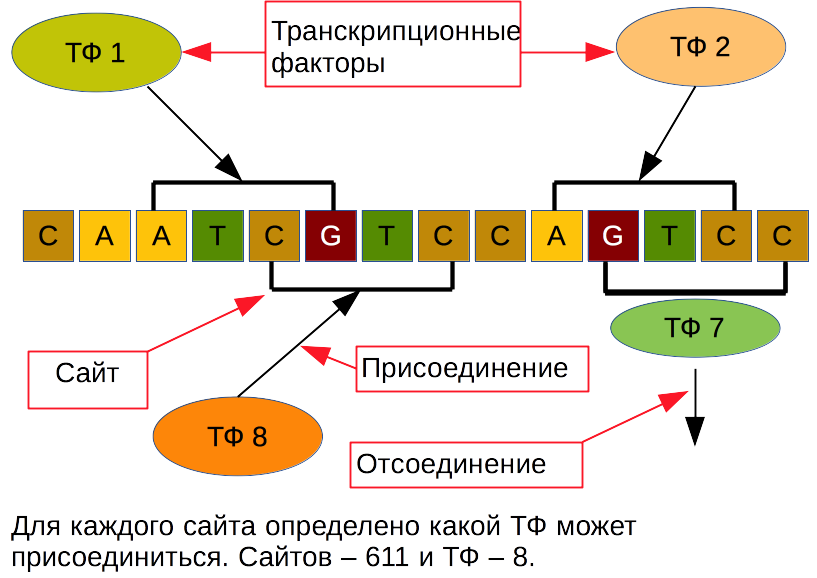
\includegraphics[width=1\linewidth]{geene_exp1}}
  \caption{Процесс присоединения и отсоединения ТФ}
  \label{fig:geene_exp1}
\end{figure}

\subsection{Транскрипция и трансляция}
Транскрипция - процесс синтеза РНК с использованием ДНК в качестве матрицы, происходящий во всех живых клетках. Как упоминалось ранее активаторами
для старта транскрипции являются белки \textbf{cad} и \textbf{bcd}. В результате транскрипции образауется молекулы РНК, которые будут участвовать в
реакции трансляции, а именно синтезировать молекулы белка.

\subsection{Диффузия и деградация}
Будем предполагать, что все молекулы у нас линейно расположены. Тогда между ядрами может происходить процесс диффузии - переход РНК в соседнее ядро.
Так же под действием внешней среды может происходить распад РНК и белка.

\begin{figure}[!h]
  \center{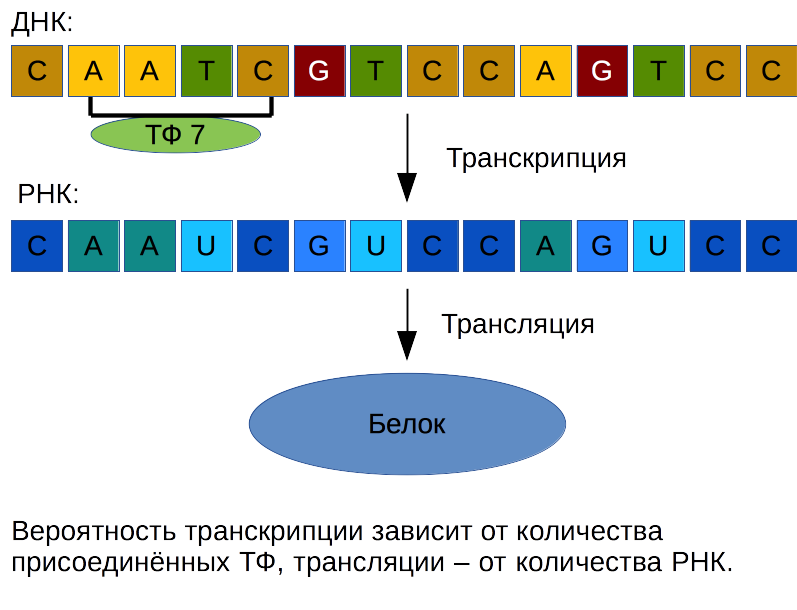
\includegraphics[width=1\linewidth]{geene_exp2}}
  \caption{Процесс транскрипции и трансляции}
  \label{fig:geene_exp2}
\end{figure}

\begin{figure}[!h]
  \center{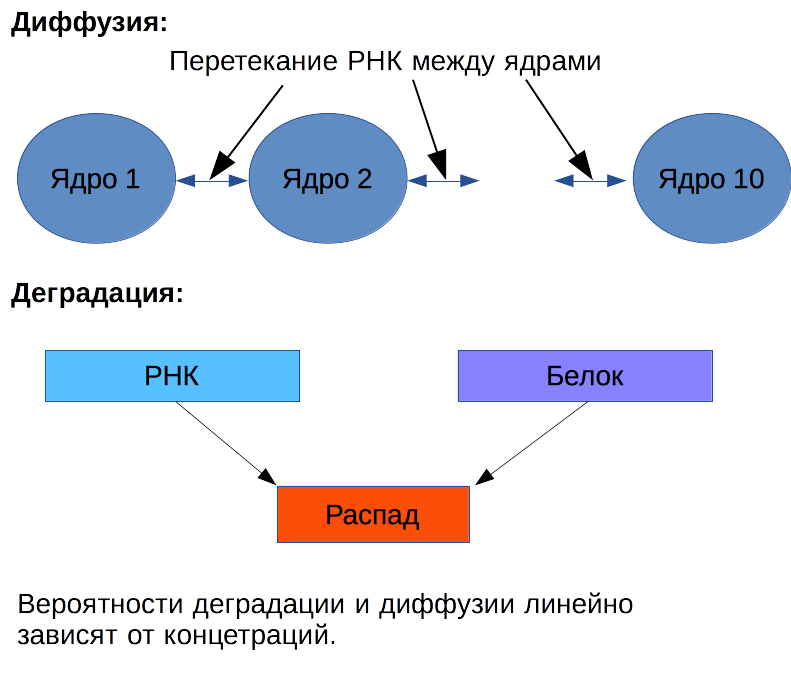
\includegraphics[width=1\linewidth]{geene_exp3}}
  \caption{Процесс диффузии и деградации}
  \label{fig:geene_exp3}
\end{figure}
